\chapter{State of Art a BTF}
\label{chapter:stateOfArt}


\section{BTF Acquisition}
\label{chapter:acquisition}

BTF acquisition is not an easy task as it requires time for acquiring and post-processing the data, and also resources are needed to create acquisition setup.
There are only a few measurement systems \cite{star2004,schwartz,dana,Kaleidoscope,Koudelka,statistical_acq} exist, but as the interest in the realistic material rendering using BTF is growing, measurement systems are developing.
In this chapter we will review how in general BTF data acquisition is made, which post-processing steps are made, and pros and cons of existing measurement systems. 
Also, we will take a look at publicly available BTF datasets.

\subsection{General Acquisition Methods}
\label{section:General_acquisition}	
All the mentioned BTF acquisition systems share the same idea in the data acquisition, i.e. capturing the appearance of a flat square slice of the material surface under varying light and camera directions.
The material surface is usually sampled over a hemisphere above the material slice as shown in Figure \ref{fig:acquisition_example}.
Depending on the material reflectance properties sampling distribution may vary, e.g. sampling distribution can be dense in regions where specular peaks in light reflection occur. 
Then, if needed uniform distribution can be made in a post-processing step with a help of interpolation \cite{haindl_visual}.

Digital cameras are used as capturing devices of the material appearance. Depending on the setup the number of cameras can vary.
 If there is only one camera \cite{star2004,statistical_acq,dana}, it usually moves around over the hemisphere above the sample with a help of robotic arm or the rail-trail system \cite{star2004}. 
 The advantage of such approach is that it is less expensive and can suit for low-budget applications.
But, the disadvantage is the positioning errors that can arise, which influence the overall measurement error. 
Depending on the application light sources can be fixed or moveable.

There are approaches which do not involve camera and light source movement at all.
Schwartz et al. \cite{schwartz} developed a novel measurement system which uses a dense array of 151 camera, which are uniformly placed on hemispherical structure.
Flashes of the cameras are used as light sources. Such setup provide high angular and spatial resolutions.

Also, Ngan et al. \cite{statistical_acq} made a setup which does not involve camera movement by placing the planar slices of the material in a form of the pyramid.
Thus, such setup captures the material appearance for 13 different camera views at once. Light directions are sampled by hand-moved electronic flash.
The disadvantage of such setup is that it provides sparse angular resolutions, but depending on the application such approach can be plausible.

The material sample is commonly flat and squared slice, which is placed the holder plate. To conduct automatic post-processing borderline markers are placed on the holder.
Those markers provide the important information for further post-processing steps such as image rectification and registration.


\begin{figure}[h]
 \centering
 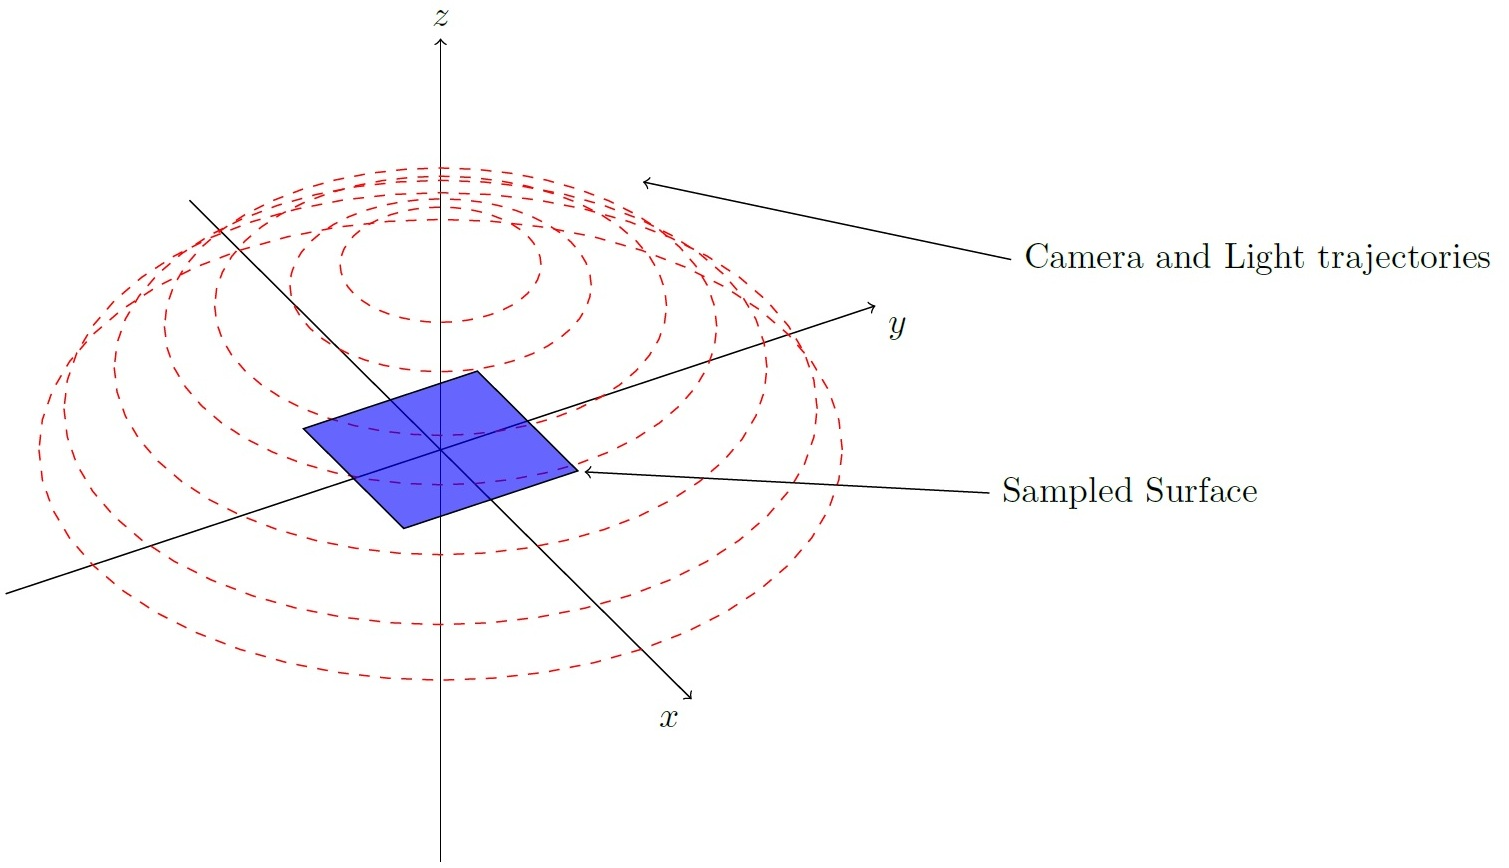
\includegraphics[width=1.0\textwidth]{figures/acquisition}
 \caption[Example of BTF measurement] {
 	{\bf Example of BTF measurement.}

	Camera and light positions share the same trajectories.
	Red dashed circles are the sample positions on the hemisphere. }
 \label{fig:acquisition_example}
\end{figure}

\subsection{Post-processing}
\label{section:Post_processing_acquisition}	
After the measurement is done, the raw data has to be further post-processed, because typically such such data is not ready for further modeling/compression or rendering.
Raw data is a set of images that are not aligned with each other and images are not mutually registered.

When the raw images are obtained under different camera angles $(\theta,\phi)$ they are perspectively distorted \cite{sattler-2003-efficient}.
Thus, sample image have to be aligned with each other and spatially registered to be further exploited.
Firstly, borderline markers that were placed around the material sample on the holder plate aid the automatic detection of the material slice.
Then, after the material slices are detected and cropped, they are ready to for mutual alignment. This process is called  \emph{rectification}. 
\emph{Rectification} is a process which involves projecting all sample images onto the plane which is defined by the frontal view, e.g. $(\theta _{o} =0,\phi _{o}=0)$.
In other words, all normals of sample images have to be aligned with their corresponding camera directions, i.e. as if all sample images were taken from frontal view $(\theta =0,\phi=0)$.
The last step is image \emph{registration}, a process of getting pixel-to-pixel correspondence between the images.
 As, all transformation were done, it is only enough to rescale all images to some equal resolution.


Even after the proper rectification and registering of the measured data, registration errors can be still present between individual camera directions \cite{haindl_visual}. 
 This happens due to structural occlusions of the material surface. Because, of such self-occlusions some geometry structures are not captured by certain camera directions, 
 but can be captured with other camera directions.
 That is why even after recti?cation images captured from completely different directions are not correctly mutually align. 
Also, registration errors can be caused both by inaccurate camera and material sample positions happened during the measurement processes.
One way to avoid artifacts in rendering caused by registration errors is to employ a compression step separately for each fixed camera positions, i.e. subsets of BTF data. 
 For instance, Sattler  \emph{et. al.} \cite{sattler-2003-efficient} has done this approach.


If needed, further processing steps can be done, for instance \emph{linear edger blending} to reduce tiling artifacts \cite{sattler-2003-efficient}.
Also, typical image processing steps may be employed, e.g. noise reduction filters. 


\subsection{Publicly Available BTF Datasets}
\label{section:Publicly_datasets}	

\begin{figure}[h]
 \centering
 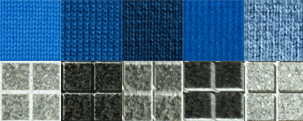
\includegraphics[width=1.0\textwidth]{figures/exampleBTF}
 \caption[Example of BTF measurement] {
 	{\bf BTF example of Bonn Database \cite{btfBonn}.}

	Example how BTF catches rich appearance of the material due to dependencies on light and camera directions. 
	Upper row is a knitted wool, lower is a graved granite stone.}
 \label{fig:exampleBTF}
\end{figure}


The accurate rendering of the material surface is highly depended on the quality of acquired data, especially for BTF.
There are several properties that are vital for reproducing quality rendering results.
The BTF datasets can be distinguished by how well image post-processing were done and how good spatial and angular resolutions are.
So, depending on the application trade-off between high and low spatial or angular resolutions is done.
 For example, some materials with a low range of reflectance may benefit from sparse resolutions, e.g. wool, plastic, etc.
 
 
A pioneer in the BTF acquisition was Dana  \emph{et. al.} \cite{curetDataBase}, who measured 61 materials with fixed light and moving camera aided by a robotic arm. 
Such procedure resulted in a set of images, which can be regarded as a subset of BTF, which is called surface light field (SLF), see Chapter \ref{section:slf}.
Data  \emph{et. al.} \emph{CUReT} database is publicly available \cite{curetDataBase}.
For each measured surface Dana  \emph{et. al.} used 205 different combinations of camera and light directions, which resulted in relatively sparse angular resolution.
 Dana's  \emph{et. al.} BTF database are not rectified, but  the authors provide image coordinates to allow their further rectification. 
 Because, of this limitations such BTF dataset usually used for computer vision purposes, i.e. texture classification  \cite{haindl_visual}.

Based on Dana  \emph{et. al.} BTF measurement system, Sattler from Bonn University made his own measuring system \cite{sattler-2003-efficient}.
 The main difference in that system is that a camera moves on a semi-circle rail around material sample.
Such setup provides spatially rectificated and mutually registered data, with reasonable angular and spatial resolutions. 
Datasets of Bonn University \cite{btfBonn} are publicly available and were used in this thesis.


 Consider Figure \ref{fig:exampleBTF}, which illustrates one of the sampled materials of Bonn database.
The measured surface is being fixed all the time on the sampler holder as shown in Figure \ref{fig:acquisition_example}. For each light position, a camera takes a shot of the material while moving from point to point of the hemisphere.
Bonn database has the same trajectory for camera and light positions, i.e. 81 positions on the hemisphere, which resulted in $81\times81=6561$ total number of acquired images.
After that the sample images were rectificated and registered, resulting in a set of images with spatial resolution $256\times256$.
Typically, the size of one uncompressed BTF is around $1.2$ Gb.



\section{BTF Data Representations}
\label{chapter:representations}




Before doing any further operation on acquired BTF it is important to chose a suitable data representation for BTF data.
Suitable presentation can enormously influence the final quality of BTF rendering and compression ratio.
\subsection{Texture Representation}
\label{chapter:texture_repr}

 The first one representation is a straightforward representation, i.e as a set of original rectified and registered textures.
Mathematically this representation expressed as

{\centering $\,\,\,\,\,\,\,BTF_{Texture}=\left \{I_{(\theta_{i} ,\phi_{i},\theta_{o} ,\phi_{o}) }  \mid  (\theta_{i},\phi_{i},\theta_{o} ,\phi_{o})\in M \right \}$\\}


where $M$ denotes a set of images $I_{(\theta_{i} ,\phi_{i},\theta_{o} ,\phi_{o})}$ measured for different light and camera directions $(i,o)$ accordingly.

Basically, $BTF_{Texture}$ is used for compression methods that do analysis on the whole sample plane.

\subsection{ABRDF Representation}
\label{chapter:abrdf_repr}

 ABRDF representation is a set of ABRDFs, one ABRDF for each sample position of the material plane. 
 ABRDF was defined in Chapter \ref{section:brdf}. In this case it is called \emph{apparent}, 
 because BTF includes effects such self-occlusions, sub-surface scattering and other complex effects which violate two basic properties of BRDF.
 
 {\centering $\,\,\,\,\,\,\,\,\,\,\,\,\,\,\,\,BTF_{ABRDF}=\left \{P_{(x) } \,\,\,\,\,\,\,\,\,\,\,\,\,\,\,\,\,\,\mid  (x)\in I_{(\theta_{i} ,\phi_{i},\theta_{o} ,\phi_{o})}\subset \mathbb{N}^{2}\right \}$ \\}
 
 $BTF_{ABRDF}$ denotes a set of $P_{(x)}$ images, i.e. ABRDF for spatial position $x$.


 $BTF_{ABRDF}$ representation allows better pixel-to-pixel comparisons, which can give a big advantage for methods that employ pixel-wise compression, e.g. BRDF based models.

Also, such arrangement provides images with lower variance \cite{haindl}, which can allow better compression results in certain scenarios, e.g. when the material surface is not smooth.
Anyway, both representations posses the same information, and any compression method can use either of them.
 
\section{BTF Compression Methods}
\label{chapter:compression_methods}



 BTF data consists of thousands of images, which means single BTF requires lots of storage space.
Bonn  Database \cite{btfBonn} consists of 8-bit PNG images with a resolution of $256\times256$ sampled for $81\times81$ different camera and light directions.
 The uncompressed data of one BTF occupies approximately 1,2 GB of space.
 To render the scene with several BTFs and to achieve acceptable frame-rates becomes practically impossible task, especially for low-end hardware.
 Also, as we intent to render BTF in a web-browser, BTF data would have to be transferred from a server to a client, which means the compact representation of BTF is inevitable in such case.
 For our scenario it is important to chose the right compression method, i.e. the one that can allows real-time decompression, high compression rate while preserving good quality, and separability of compressed BTF data.
 Separability is needed for real-time streaming in a web-browser.  
 As the data is streamed in small chunks and at some point it is important to have an option to render the preview of BTF based on the partial data.

There are different types of methods applied for compressing the BTF. Those methods can be categorized the following way:

\begin{itemize}
  \item \emph{Analytic methods} group, where BTF is represented by analytic BRDF models. 
Analytic BRDF models are the functions which fit separately each texel of BTF. Such functions store few parameters, thus high real-time performance is easily achieved.
However, these group of methods can suffer from decreased quality \cite{haindl}. Also, it is hard to change parameters in order to control the visual quality. Chapter  \ref{section:analytic_methods}.
   \item \emph{Statistical methods}, which belong to methods that reduce dimensionality based on  statistics, for instance based linear basis decompression method such as PCA (Principal component analysis). 
    PCA based methods are frequently used, because its parameters directly correspond to the trade-off between compression ratio and reconstruction quality.
    Also, PCA is frequently a basis point for some more sophisticated methods \cite{webglbtfstreaming}. Chapter \ref{section:stat_methods}.
   \item \emph{Probabilistic models}, which can spatially enlarge BTF to any arbitrary size without visible discontinuities and extremely compress the original BTF.
   However, the resulted quality usually suits for flat surfaces and there are problems of implementing in GPU for real-time rendering. Chapter \ref{section:prob_methods}.
 \end{itemize}



 \subsection{Analytic methods}
\label{section:analytic_methods}	
 This group of methods take advantage of ABRDF representation of BTF. 
 There is a large number of techniques which allow compactly represent BRDF, which in essence can be also applied for ABRDF.
 Each texel of BTF, i.e. spatial position of surface are represented as ABRDF. Each of these ABRDFs can be modeled and compressed by any BRDF model.
 
One of the possible ways to model ABRDF is to use \emph{Polynomial Texture  Mapping} (PTM) approach.
Malzbender  \emph{et. al.} \cite{PTM} used this approach which allows for high compression rates and generally good quality. 
However, PTM requires to compute specular and diffuse effects separately. 
PTM model assumes that the input surfaces has to be either diffuse or their specular contribution is separated beforehand.
For BTF it can be quite difficult to separate specular highlights \cite{haindl}.

Haindl  \emph{et. al.} \cite{haindl} applied PTM for a fixed camera positions of BTF, i.e. for reflectance fields (RF).
General formula looks the following way (PTM RF):

{\centering$R_{o}(r,i)\approx a_{0}(r)u_{x}^2+a_{1}(r)u_{y}^2+a_{2}(r)u_{x}u_{y}+a_{3}(r)u_{x}+a_{4}(r)u_{y}+a_{5}(r)$\\}

 where $R_{o}$ is approximated RF for fixed camera direction $o$ and $u_{x},u_{y}$ are projections of the normalized light vector into the local coordinate system $r=(x,y)$.
 Set of all possible $R_{o}$ is the number of all camera positions, i.e. $n_{o}$. 
 Coefficients $a_{p}$ are fitted by the use of \emph{singular value decomposition} SVD for each $R_{o}$ and parameters stored as a spatial map referred to as a PTM.
 
 However, Malzbender  \emph{et. al.} \cite{PTM} claims that this method produce considerable errors for high grazing angles. 
 But, nevertheless this method enables fast rendering and generally suited for smooth material surfaces.
 
 Another model which produces slightly better visual quality is the polynomial extension of one-lobe Lafortune model (PLM) \cite{haindl}.
One-lobe Lafortune model (LM) looks the following way \cite{plm}:

{\centering$Y_{o} (r,i) = \rho_{o,r}(C_{o,r,x}u_{x}+C_{o,r,y}u_{y}+C_{o,r,z}u_{z})_{ }^{n_{o,r}}$\\}

where $w_{i}(\theta_{i}, \phi_{i})=[u_{1},u_{2},u_{3}]^{T}$ is a unit vector pointing to light position.
Parameters $\rho,C_{x},C_{y},C_{z},n$ can be computed with a Levenberg-Marquardt non-linear optimisation algorithm \cite{plm}. 
During testing of this model Filip and Haindl \cite{plm} claim that LM produce unsatisfactory results for complex ABRDFs.
 Thus, the polynomial extension of one-lobe Lafortune was introduced (PLM RF):

{\centering$R_{o}(r,i)\approx  \sum_{j=0}^{n} a_{r,o,i,j}Y_{o}(r,i)^j$\\}



PLM RF solves the problem of bad quality for grazing angles and improves the rendering quality compared to PTM RF.
However, statistical based methods produce even better quality compared to above methods but with lower compression rates \cite{haindl}.



  \subsection{Statistical methods}
\label{section:stat_methods}
 Statistical methods group belong to the context of pattern recognition and aimed to make benefit from the statistical properties of a BTF \cite{schneider2004}.
This group of methods mostly based on a dimensionality reduction of a data, while preserving the most important information.
The goal of the dimensionality reduction is to find a new basis which would represent the data with less dimensions and at the same time preserving the important features of the original data.
 The size of the data with the new basis will be decreased.

One of the popular methods used for a BTF compression which belong to this group of methods is \emph{Principal component analysis} (PCA) \cite{Bishop,schneider2004,haindl,webglbtfstreaming,sattler-2003-efficient,mueller-2003-compression,gpu_gems}.
PCA is a linear transformation of the data to a new basis, where each new coordinate (variable) is called \emph{principal component} \cite{Bishop}.
Each new coordinate are mutually orthogonal, i.e. uncorrelated. Components are sorted by decreasing variance, i.e. first component posses the greatest variance compared to other components, 
second one holds the second greatest variance and so on. The last components which hold small variations are discarded, because they do not hold important information.
The ones that are left for a new basis are called \emph{principal components}.
In more detailed form PCA method is explained in Chapter \ref{section:pca}, which was used in our work.

The reason why PCA is a popular approach for compressing BTF are because of the following reasons. 
Firstly, PCA allows for a strong correspondence between the number of components and the decompression error.
 The correspondence lies in the amount of components used.
 The bigger quantity of components are used to gain better decompression error, and vise-verse the smaller number of components gives better compression ratio, but worse decompression error.
 This makes easier to regulate the estimated parameters, i.e. to do a trade-off between a rendering quality and a compression ratio.
Secondly, reasonable compression ratio along with low decompression error can be achieved, e.g. compression ratio $1:100$ with an average decompression error 2\%- 4\% \cite{schneider2004,haindl}.
Thirdly, PCA is suitable for real-time decompression for average GPU \cite{schneider2004,haindl}. 
It is suitable, because decompression of one single pixel is not depended on the other pixels, which suits the nature of GPU.
 And computation of a single pixel for PCA decompression on the GPU is done by means of linear combination of estimated PCA parameters, so the speed of decompression depends on number of components used.
 
 There exist different methods based on PCA, i.e. PCA \emph{Reflactance Field} (RF), PCA BTF and local PCA (LPCA) \cite{sattler-2003-efficient,schneider2004,mueller-2003-compression, haindl}.
 Sattler \emph{et. al.} \cite{sattler-2003-efficient} developed PCA RF. 
 This method ensures a pixel position coherence, by employing PCA per camera direction. 
 The advantage is that on average 8 components are enough to get good quality results with decompression error  2\%- 4\%.
 On the other hand, PCA BTF method, which does PCA on all camera directions at once, requires on average 41 components \cite{haindl}.
 M{\"u}ller  \emph{et. al.} \cite{schneider2004} improved PCA BTF by exploiting the vector quantization technique and applying PCA  for resulted clusters.
 The name of this method is local PCA (LPCA). On average this method requires 19 components \cite{haindl}.
 Even though compression ratio of PCA RF is lower than PCA BTF and LPCA, it is less computational demanding.


Last but not least, any PCA method is suitable for streaming purpose, as it is possible to stream components separately and progressively enhance the rendering quality. 






 \subsection{Probabilistic models}
\label{section:prob_methods}

Compression methods based on probabilistic models \cite{car_model,gmrf_model,haindl}
 provide much higher compression rate than most others methods and allow for a seamless enlargement of textures of any size \cite{haindl}. 
Usual compression  compression ratio achieved by such models are $1:6-8\times 10^{4}$.
But, the visual quality of rendered results suits best for smooth material surfaces, while materials with high frequencies can appear flat using probabilistic methods \cite{haindl}.
Also, these type of models can be problematic for implementation on low-end GPUs. 
The problem arise in shaders, when probabilistic model requires information of spatial neighbours to synthesize the texture \cite{gmrf_model,haindl}.
Even though solutions exists  how to handle such problem, e.g. take advantage of Framebuffers Objects, which allow access for previously rendered results \cite{haindl}.
Such solution may be time-consuming for low-end GPUs.

A common algorithm that employs probabilistic model combines a material range map and synthetic smooth texture produced by a probabilistic model.
Range map is a monochrome image that stores the depth of each spatial position of the material surface \cite{gmrf_model}.
If the synthetic texture is larger than range map, it can be enlarged using the Roller technique\cite{btfroller}.
Currently there are available several probabilistic models, i.e. Gaussian Markov Random Field (GMRF) and  Causal Autoregressive (CAR) models \cite{haindl,Bishop}.
Commonly these models are 3D models which further factorized and modelled by less dimensional models, i.e. by a set of 2D models.
2D models requires less parameters to store. Such models are very complex, because they can store up to thousand 2D models \cite{haindl_visual}.
The learning process of such models is not easy as well, because it requires large training data set. 
Thus, probabilistic models can be applied to some simpler materials, e.g. smooth materials. 
Materials with high frequencies can result in a flat look, as shown by Haindl  \emph{et. al.} \cite{haindl}.
Also, the set of 2D models has to be trained simultaneously, thus it demands high computational effort.



